\documentclass[11pt,border=20pt]{standalone}
\usepackage{tikz}
\usepackage[T1]{fontenc}
\usepackage{tgheros}
\renewcommand{\familydefault}{\sfdefault}
\usepackage{inconsolata}
\usetikzlibrary{shapes.geometric, arrows.meta, positioning, shadows, decorations.pathreplacing, calc, fit, backgrounds}

% Define colors
\definecolor{phase1color}{RGB}{33, 150, 243}
\definecolor{phase2color}{RGB}{76, 175, 80}
\definecolor{phase3color}{RGB}{255, 167, 38}
\definecolor{phase4color}{RGB}{156, 39, 176}
\definecolor{darkgray}{RGB}{66, 66, 66}

% Define styles
\tikzstyle{phase_box} = [rectangle, rounded corners=8pt, minimum width=5cm, minimum height=1.5cm, text centered, line width=2pt, font=\sffamily\large\bfseries, drop shadow={shadow xshift=2pt, shadow yshift=-2pt, opacity=0.3}]
\tikzstyle{arrow} = [ultra thick,->,>=stealth, darkgray, line width=3pt]
\tikzstyle{title} = [font=\sffamily\Huge\bfseries, darkgray]
\tikzstyle{description} = [font=\sffamily\footnotesize, darkgray, text width=8.2cm, align=left]

\begin{document}
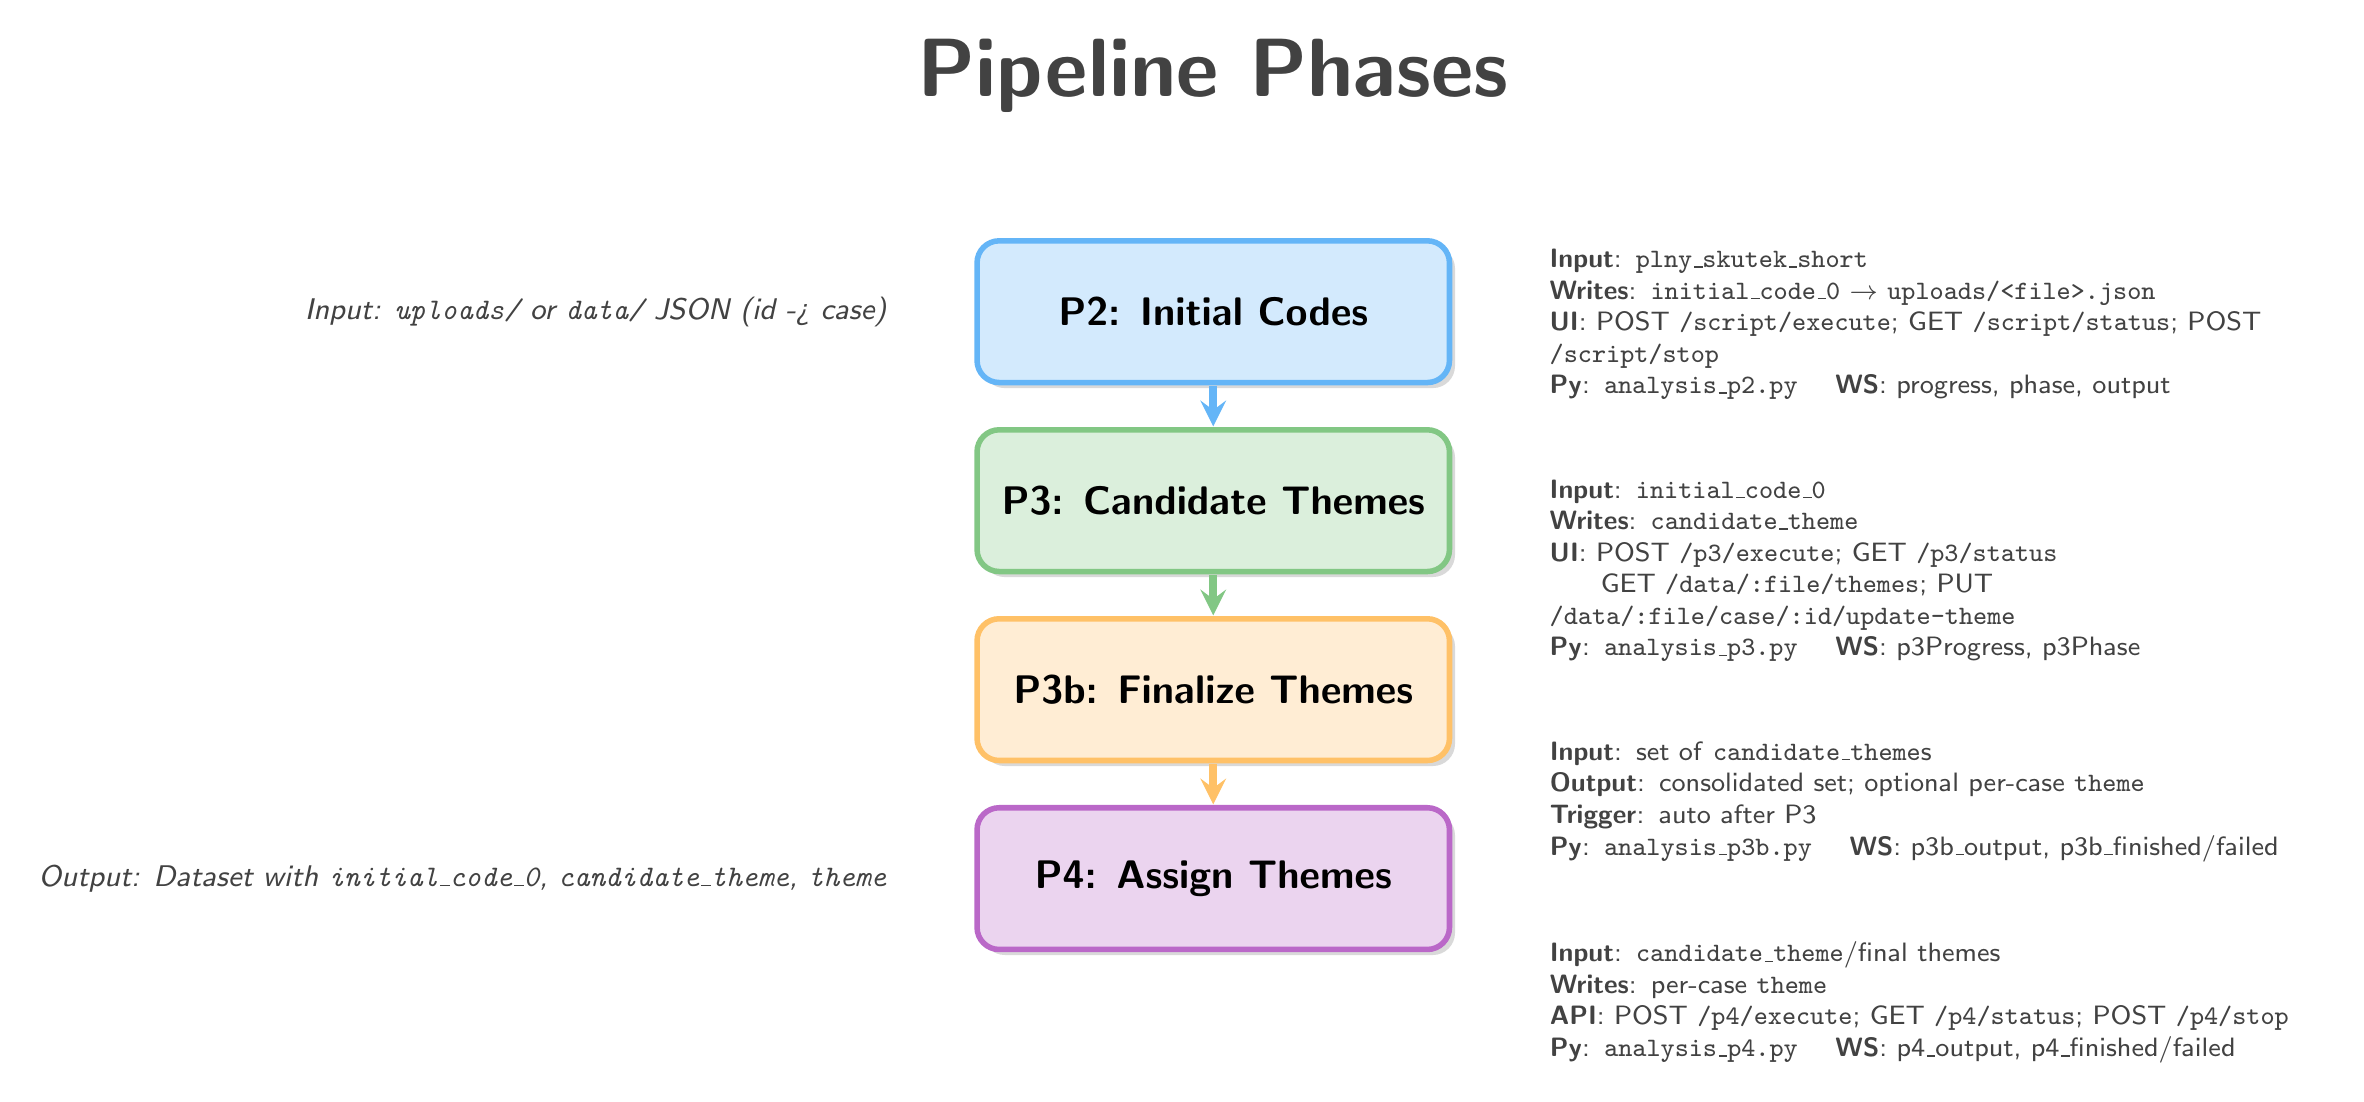
\begin{tikzpicture}[scale=1.2, transform shape]

% Title
\node[title] at (0, 6) {Pipeline Phases};

% Phase boxes with gradient-like effects
\node[phase_box, fill=phase1color!20, draw=phase1color!70] (p2) at (0, 3.5) {P2: Initial Codes};
\node[phase_box, fill=phase2color!20, draw=phase2color!70] (p3) at (0, 1.5) {P3: Candidate Themes};
\node[phase_box, fill=phase3color!20, draw=phase3color!70] (p3b) at (0, -0.5) {P3b: Finalize Themes};
\node[phase_box, fill=phase4color!20, draw=phase4color!70] (p4) at (0, -2.5) {P4: Assign Themes};

% Arrows between phases
\draw[arrow, phase1color!70] (p2.south) -- (p3.north);
\draw[arrow, phase2color!70] (p3.south) -- (p3b.north);
\draw[arrow, phase3color!70] (p3b.south) -- (p4.north);

% Descriptions stacked in a single right column to avoid overlap
\coordinate (descStart) at ($ (p2.north east) + (0.9cm,0) $);
\node[description, anchor=north west] (p2d) at (descStart) {
  \textbf{Input}: \texttt{plny\_skutek\_short}\\
  \textbf{Writes}: \texttt{initial\_code\_0} $\rightarrow$ \texttt{uploads/<file>.json}\\
  \textbf{UI}: POST \texttt{/script/execute}; GET \texttt{/script/status}; POST \texttt{/script/stop}\\
  \textbf{Py}: \texttt{analysis\_p2.py} \quad \textbf{WS}: progress, phase, output
};

\node[description, anchor=north west] (p3d) at ($ (p2d.south west) + (0,-0.6cm) $) {
  \textbf{Input}: \texttt{initial\_code\_0}\\
  \textbf{Writes}: \texttt{candidate\_theme}\\
  \textbf{UI}: POST \texttt{/p3/execute}; GET \texttt{/p3/status}\\
  \phantom{\textbf{UI}:}\, GET \texttt{/data/:file/themes}; PUT \texttt{/data/:file/case/:id/update-theme}\\
  \textbf{Py}: \texttt{analysis\_p3.py} \quad \textbf{WS}: p3Progress, p3Phase
};

\node[description, anchor=north west] (p3bd) at ($ (p3d.south west) + (0,-0.6cm) $) {
  \textbf{Input}: set of \texttt{candidate\_theme}s\\
  \textbf{Output}: consolidated set; optional per-case \texttt{theme}\\
  \textbf{Trigger}: auto after P3\\
  \textbf{Py}: \texttt{analysis\_p3b.py} \quad \textbf{WS}: p3b\_output, p3b\_finished/failed
};

\node[description, anchor=north west] (p4d) at ($ (p3bd.south west) + (0,-0.6cm) $) {
  \textbf{Input}: \texttt{candidate\_theme}/final themes\\
  \textbf{Writes}: per-case \texttt{theme}\\
  \textbf{API}: POST \texttt{/p4/execute}; GET \texttt{/p4/status}; POST \texttt{/p4/stop}\\
  \textbf{Py}: \texttt{analysis\_p4.py} \quad \textbf{WS}: p4\_output, p4\_finished/failed
};

% Alternative vertical layout with annotations
% Data flow indicators
\node[font=\sffamily\small\itshape, darkgray, left=0.8cm of p2] {Input: \texttt{uploads/} or \texttt{data/} JSON (id -> case)};
\node[font=\sffamily\small\itshape, darkgray, left=0.8cm of p4] {Output: Dataset with \texttt{initial\_code\_0}, \texttt{candidate\_theme}, \texttt{theme}};

\end{tikzpicture}
\end{document}